%*
%* Seven Kingdoms: Ancient Adversaries
%*
%* Copyright 1997,1998 Enlight Software Ltd.
%* Copyright 2018 Timothy Rink
%*
%* This program is free software: you can redistribute it and/or modify
%* it under the terms of the GNU General Public License as published by
%* the Free Software Foundation, either version 2 of the License, or
%* (at your option) any later version.
%*
%* This program is distributed in the hope that it will be useful,
%* but WITHOUT ANY WARRANTY; without even the implied warranty of
%* MERCHANTABILITY or FITNESS FOR A PARTICULAR PURPOSE.  See the
%* GNU General Public License for more details.
%*
%* You should have received a copy of the GNU General Public License
%* along with this program.  If not, see <http://www.gnu.org/licenses/>.
%*
%*

\chapter[The Village]{{\Huge T}HE {\Huge V}ILLAGE}

\textbf{\textswab{\huge{C}}lick} on any one of the small houses in your first Village. When you do, you will see the Village Command Bar to the right of the main screen.

\begin{center}
    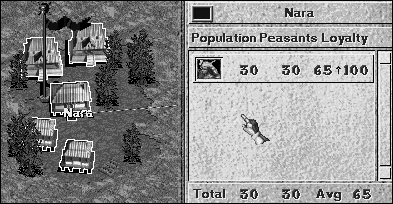
\includegraphics[width=0.9\linewidth]{Ivillage} % Original size.
\end{center}

\section{\textsf{Village Demographics}}

\index{demographics of village}
\index{villages!demographics}

\subsection{\textsf{Population/Nationality}}

\textswab{\huge{T}}he number on the lower left shows the total number of people in the selected Village. They are divided into their various national groupings, which you can distinguish by the small pictures on the far left. As long as you have not disabled the Help feature, holding your cursor over one of the small pictures for a few seconds will pop up a text bubble telling you which nationality it is.

Although there may be up to seven different nationalities in Villages that you will later build, absorb, or conquer, in your first Village there will be only one.

The style of houses in Villages will give you a quick idea as to what nationalities reside there.

To see what types of houses belong to which nationalities, see the house images in \textbf{Chapter 14}.

Populations in Villages will increase over time up to a maximum of 60. The rate of increase will not be the same for all Villages because Villages which have access to a steady supply of consumer goods will grow faster than those without. Higher standards of living induce higher growth rates.

See \textbf{Chapter 20} for Economic Strategy Tips.

\subsection{\textsf{Peasants}}

\index{peasants}

\textswab{\huge{A}}t the bottom of the middle column, you will see the total number of Peasants at work in the fields of this Village. They can either be left toiling in the fields, trained in various skills, ordered to work in other jobs, or sent out to be instructed in the ways of war.

Because Peasants grow all of the food for your empire, it is important to leave enough of them working in the fields. Each Peasant will produce 30 units of food per year, and each subject of your kingdom will consume 10 units per year. Thus, to maintain a sufficient food supply, you must have at least one Peasant for every three subjects.

\subsection{\textsf{Loyalty}}

\index{loyalty}

\begin{wrapfigure}{r}{0.4\textwidth}
    \vspace{-20pt}
    \begin{center}
        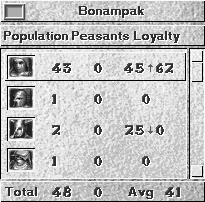
\includegraphics[width=0.4\textwidth]{Ivillage_peasants} % Original size.
    \end{center}
    \vspace{-20pt}
\end{wrapfigure}

These numbers (on the far right) show the level of Loyalty to your kingdom for each Nationality in a Village. The arrows indicate whether this Loyalty is increasing or decreasing.

On the bottom right, you can see the average Loyalty Level for all of the Nationalities in the Village.

If the Loyalty of a Nationality in one of your Villages falls to 30 or below, there will be a danger of revolt in that group.

Low Loyalty levels may also have negative impacts other than open revolt. Individual Villagers may leave your Villages for other Kingdoms, Independent Villages, or for unknown regions, although they will be most likely moved to a Village that is Linked to their present home.

\textbf{Loyalty Levels are positively influenced by:}

\begin{changemargin}{.5cm}{0cm}
Residential Harmony, which itself is a result of having a single Nationality in a Village rather than multiple Nationalities. The Villagers being of the same Nationality as the King.

A high Reputation for your Kingdom will help increase the Loyalty Level of all Villagers.

Having a General, in a Fort Linked to the Village, who is of the same Nationality as the Villagers. If the General has a high Leadership Level, the effect will be increased. If the General’s Nationality is the same as the King’s, the effect will be increased by an additional 50\%.
\end{changemargin}

\textbf{Loyalty Levels are negatively affected by:}

\begin{changemargin}{.5cm}{0cm}
Having a Fort from another Kingdom within Linking distance of your Village. If the rival General in that Fort is of the same Nationality as your Villagers, the effect will be increased, especially if he has a high Leadership Level.

A low Reputation for your Kingdom will hold down the Loyalty Level of all Villagers.

Recruiting Villagers or conscripting them directly into a Fort will lower a Village’s Loyalty somewhat for each Villager Recruited.
\end{changemargin}

\textbf{Loyalty Levels of Workers:}

\begin{changemargin}{.5cm}{0cm}
Since all Workers reside in Villages, their Loyalty Levels are reflected in the Loyalty Level of the Villages. This differs from Soldiers who reside inside Forts.
\end{changemargin}

\subsection{Quality of Life}

\index{quality of life}

\textswab{\huge{H}}aving a high Quality of Life in your Villages will cause their population to grow faster. With a large population, you will have an abundance of the most precious resource in \textit{Seven Kingdoms: Ancient Adversaries}, People.

Even the most ruthless of tyrants will benefit from improving his subjects’ lifestyle. If you wish your Villagers to have a high Quality of Life, you must make sure that they have access to consumer goods in Markets. The greater the quantity and variety of goods for them to buy, the higher their Quality of Life will be.

\section{\textsf{Commanding Your Peasants}}

\index{commanding peasants}

\subsection{\textsf{Recruit}}

\index{recruiting peasants}

\begin{wrapfigure}{r}{0.1\textwidth}
    \vspace{-20pt}
    \begin{center}
        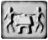
\includegraphics[width=0.1\textwidth]{Trecruit}
    \end{center}
    \vspace{-20pt}
\end{wrapfigure}

\textswab{\huge{W}}ith this command, you order your peasants out of their Villages and assign them where you will. Have a care, though; Peasants resent this conscription, and there is therefore a small decrease in Village loyalty for each peasant recruited.

The rate of the decrease will depend upon the frequency of your Recruiting. Infrequent Recruiting will result in a lower Loyalty decrease than frequent Recruiting.

This tile will no longer be available if there are no more Peasants left in your Village.

\subsection{\textsf{Moving between Villages}}

\index{moving between villages}
\index{villages!moving between}

\begin{wrapfigure}{r}{0.6\textwidth}
    \vspace{-20pt}
    \begin{center}
        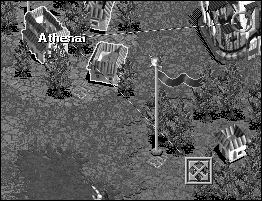
\includegraphics[width=0.6\textwidth]{Ivillage_villagelink} % Original size.
    \end{center}
    \vspace{-20pt}
\end{wrapfigure}

\textswab{\huge{I}}f you settle a new Village within Linking distance of an older Village, you will, when either of the Villages is selected, see a bright pink 4-Arrow Icon at the end of the Link.

If you wish to move Villagers from one Village to another \textbf{\textit{without}} suffering the decrease in Loyalty that you get when Recruiting Villagers, you may \textbf{Right-Click} on the Pink 4-Arrow Icon. One Villager at a time will then move from the selected Village into the Village under the Icon when \textbf{Left-Clicking}; when \textbf{Right-Clicking}, ten Villagers will move.

\subsection{Train}

\index{training peasants}

\begin{wrapfigure}{r}{0.1\textwidth}
    \vspace{-20pt}
    \begin{center}
        
\includegraphics[width=0.1\textwidth]{Ttrain}
    \end{center}
    \vspace{-20pt}
\end{wrapfigure}

\textswab{\huge{A}}ny Peasant may be trained in any of several useful skills. Training each unit will cost \$30. At the end of his training, which will take five days, the new Worker will have a skill level of 20. This skill will soon grow if he is put to work. Non-trained units who go to work will also see their skill levels increase, although from a starting level of 10.

Some workers are born with an inborn potential that outstrips that of their peers. Their Skill Levels will increase at a faster rate.

\subsubsection{\textsf{How to Train a Unit}}

\textswab{\huge{F}}irst select the Village where you want the Peasant to be trained in a new skill.

\textbf{NOTE:} If you have no Fort linked to the Village, or if you have a Fort that is not staffed with a General or King, this Tile will not be available, and you will be unable to train anyone.

Then \textbf{Click} on the \textbf{Train Tile} (above). The six Training Categories will appear on the right of your screen.

\textbf{Click} on the skill that you want, and one Peasant will begin training in his new profession.

\begin{wrapfigure}{r}{0.4\textwidth}
    \vspace{-20pt}
    \begin{center}
        
\includegraphics[width=0.4\textwidth]{Itrainprogress} % Original size.
    \end{center}
    \vspace{-15pt}
\end{wrapfigure}

You may cancel the training of a unit by \textbf{Clicking} on the large \textbf{X} to the right of the blue progress bar.

\subsubsection{\textsf{How to Train more than one Unit at a time}}

\begin{wrapfigure}{r}{0.35\textwidth}
    \vspace{-20pt}
    \begin{center}
        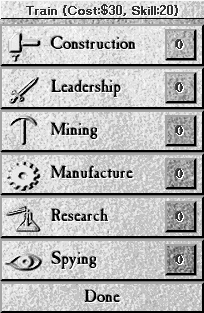
\includegraphics[width=0.35\textwidth]{Itrain} % Original size.
    \end{center}
    \vspace{-20pt}
\end{wrapfigure}

\textswab{\huge{T}}o the right of the Skill description, you will see another, smaller button with a number on it.

\textbf{Click} on this button repeatedly until it shows the number of Peasants that you want to train in a new skill.

\textbf{Right-Clicking} on the number button will decrease the number by one.

You may set numbers for more than one skill at a time.

When you are finished, \textbf{Click} on the \textbf{Done Button}. The Workers and/or Soldiers with their new skills will exit the Village one at a time as they are trained.

All Trained Units will begin with a Skill Level of 20.

Trained Units; Skill Levels will steadily increase, but only while they are at work. “At work” does not only mean being in their place of work; they must have something to do while there. For example, if a Factory has no Raw Materials to work with, then the skill of the workers will not increase.

\subsubsection{\textsf{Construction}}

\index{skills!construction}
\index{construction skill}

\begin{wrapfigure}{r}{0.1\textwidth}
    \vspace{-20pt}
    \begin{center}
        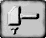
\includegraphics[width=0.1\textwidth]{Thammer}
    \end{center}
    \vspace{-20pt}
\end{wrapfigure}

\textswab{\huge{A}} unit trained in Construction is necessary to supervise the erection of most Buildings. Although other trained units (see below) may build certain structures, a unit trained in Construction will be able to build them all.

Construction of a Building will be suspended if the building is under attack.

In order to repair a damaged building, a worker trained in Construction must be assigned to it. To do this, send a selected Construction unit into any Building with a \textbf{Right-Click}.

The speed of a building’s construction or repairs will depend on the Skill Level of the Construction worker. The higher his skill, the faster he will build or repair.

\subsubsection{\textsf{Leadership}}

\index{skills!leadership}
\index{leadership skill}

\begin{wrapfigure}{r}{0.1\textwidth}
    \vspace{-20pt}
    \begin{center}
        
\includegraphics[width=0.1\textwidth]{Tleadership}
    \end{center}
    \vspace{-20pt}
\end{wrapfigure}

\textswab{\huge{A}} unit trained in Leadership serves as a soldier in your kingdom’s military, or be promoted to General. Upon completion of Leadership training, a unit will have an initial skill of 20 in both Leadership and Combat. If later promoted to Generals, trained leaders are also effective in helping your Empire to absorb independent Villages. Units trained in Leadership will be able to erect Forts, and having been used for this, they will immediately be assigned there when construction is complete.

\subsubsection{\textsf{Mining}}

\index{skills!mining}
\index{mining skill}

\begin{wrapfigure}{r}{0.1\textwidth}
    \vspace{-20pt}
    \begin{center}
        
\includegraphics[width=0.1\textwidth]{Tmining}
    \end{center}
    \vspace{-20pt}
\end{wrapfigure}

\textswab{\huge{A}} unit trained in Mining will begin as a more productive Miner, producing more raw materials for your factories than an untrained worker can. Units trained in Mining will also be able to dig Mines. If they are used for this, they will immediately be assigned there to begin their work.

\begin{wrapfigure}{r}{0.1\textwidth}
        \begin{center}
        
\includegraphics[width=0.1\textwidth]{Tmanufacturing}
    \end{center}
    \vspace{-20pt}
\end{wrapfigure}

\subsubsection{\textsf{Manufacturing}}

\index{skills!manufacturing}
\index{manufacturing skill}

\textswab{\huge{A}} unit trained in Manufacturing will begin working in your Factories and War Factories as a more productive worker than one who is untrained. Units trained in Manufacturing will be able to erect Factories and War Factories. If they are used for this, they will immediately be assigned there to begin production.

\begin{wrapfigure}{r}{0.1\textwidth}
        \begin{center}
        
\includegraphics[width=0.1\textwidth]{Tresearch}
    \end{center}
    \vspace{-20pt}
\end{wrapfigure}

\subsubsection{\textsf{Research}}

\index{skills!research}
\index{research skill}

\textswab{\huge{A}} unit trained in Research will aid you in discovering the technologies needed to build Advanced Weapons and Ships.

Units trained in Research will be able to erect Towers of Science. If they are used for this, they will immediately be assigned there to begin their research.

\subsubsection{\textsf{Spying}}

\index{skills!spying}
\index{spying skill}

\begin{wrapfigure}{r}{0.1\textwidth}
    \vspace{-20pt}
    \begin{center}
        
\includegraphics[width=0.1\textwidth]{Tspy}
    \end{center}
    \vspace{-20pt}
\end{wrapfigure}

\textswab{\huge{A}} unit trained in Spying will be able to penetrate enemy Villages, influencing the Villagers’ loyalty, and give you all the information on the population that your enemy himself possesses. Spies may penetrate firms, quietly sabotaging production.

% Drinking in enemy Inns, ...

Drinking in enemy Inns, they may be recruited and put into an important position in their society. They may even penetrate enemy Forts, giving you unrivaled intelligence on Combat levels, and giving your Spy the opportunity to assassinate a General or a King. 

For many more details on Spies and Espionage, see \textbf{Chapter 13}.

\subsubsection{\textsf{More Details on all Trained Units}}

\textswab{\huge{W}}hen outside and selected, all of your trained units will show a small icon above their heads denoting their particular specialty. These icons are the same as those appearing on the Train menu.

When you place your cursor over subjects of another kingdom, you will also be able to see their particular skill.

Any enemy unit without a Sword Icon is a civilian. It is good to know this as it will hurt your Kingdom’s Reputation if you attack civilians.

You should realize that your King and your Generals are easily recognizable to both friends and foes. It is therefore imperative that you protect these valuable units as best you can, because in battle, both human and computer controlled foes will probably attempt to slay your commanders first.

The productivity levels of all trained workers who have been injured will decline in proportion to their injury. Injury will also slow down the speed of their training.

The same rule applies to training soldiers. If a fort’s commander is injured, the training of his Troop will be slowed, as will any increase to his own Leadership skill.

When a unit is sent to work in a building that already has a full complement of workers, he will replace the worker with the lowest skill level. That replaced worker will return to a Linked Village where he will live as a Peasant.

If you send a soldier into an already full Fort, one soldier from the Fort will then exit and stand outside. He will not Settle in a Village.

\begin{wrapfigure}{r}{0.5\textwidth}
    \vspace{-20pt}
    \begin{center}
        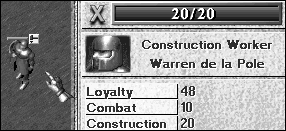
\includegraphics[width=0.5\textwidth]{Ipeasant} % Original size.
    \end{center}
    \vspace{-20pt}
\end{wrapfigure}

You may easily view the identity and other pertinent information on any unit by selecting it. The unit’s information will be displayed on the right. \\ % adds vspace due to wrapfig.

\section{\textsf{Collect Tax}}

\index{collecting taxes}
\index{taxes}

\textswab{\huge{T}}axes are yours to command from your people. In \textit{Seven Kingdoms: Ancient Adversaries}, there are two types of taxes. The Yearly Tax will be collected every January 1st from every person living in your Villages.

\begin{wrapfigure}{r}{0.1\textwidth}
    \vspace{-20pt}
    \begin{center}
        
\includegraphics[width=0.1\textwidth]{Ttax}
    \end{center}
    \vspace{-20pt}
\end{wrapfigure}

Special Taxes may also be collected from each person living in a selected Village. When a Special Tax is collected, the Loyalty Level of all Villagers in the selected Village will decrease. The amount of the decrease will depend upon how often your tax collectors come calling. Collecting Taxes several times in quick succession will result in far greater loss of Loyalty than taxing over a greater period of time.

There will be no decrease in loyalty for the Yearly Tax.

\begin{wrapfigure}{r}{0.3\textwidth}
    \vspace{-20pt}
    \begin{center}
        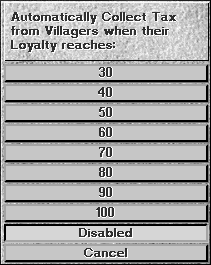
\includegraphics[width=0.3\textwidth]{Iautotax} % Original size.
    \end{center}
    \vspace{-20pt}
\end{wrapfigure}

\textbf{Auto-Taxing a Single Village}: If you \textbf{Right-Click} on the \textbf{Tax Tile}, you will be presented with a list of Loyalty Levels. By \textbf{Clicking} on one of these, you will automatically collect a Special Tax from the selected Village whenever their Loyalty reaches this level.

\textbf{Auto-Taxing All Villages}: By \textbf{Right-Clicking} on one of the numbers, instead of \textbf{Clicking}, you will, in the future, collect a Special Tax from every one of your Villages when their average Loyalty Level reaches the selected level.

This will also apply to new Villages when they are settled.

\subsection{\textsf{Grant}}

\index{grants}

\begin{wrapfigure}{r}{0.1\textwidth}
    \vspace{-20pt}
    \begin{center}
        
\includegraphics[width=0.1\textwidth]{Tgrant}
    \end{center}
    \vspace{-20pt}
\end{wrapfigure}

\textswab{\huge{G}}rants are the exact opposite of taxes. If you find some of your Villages’ Loyalty lacking, common peasants and workers are easily placated by spreading a little of your excess treasure around. Assuming that you have abundant funds, providing Grants to Villages around your Empire to ensure complete loyalty makes very good sense.

Each Grant will distribute \$10 to every Villager in the selected Village. The Villagers will then show an increase in their Loyalty Levels. The amount of increase will vary depending upon how often you Grant money to them. Issuing several Grants in rapid succession will have less effect than spreading your generosity out over a greater span of time.

Grants may also be issued to Independent Villages if you have a Fort Linked to them and staffed with a General or your King. Each Grant to an Independent Village will cost you \$30 per Villager. These Grants will quickly lower the resistance of that Village to your rule, but at great cost to you.

You may also Grant money to Villagers of other Kingdoms if you have a staffed Fort Linked to their Village, and the other kingdom does not. These Grants will lower the Loyalty Level of those Villagers to their King.

\begin{wrapfigure}{r}{0.3\textwidth}
    \vspace{-20pt}
    \begin{center}
        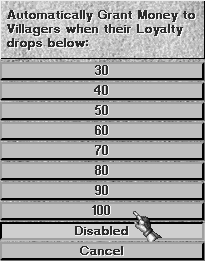
\includegraphics[width=0.3\textwidth]{Iautogrant} % Original size.
    \end{center}
    \vspace{-20pt}
\end{wrapfigure}

\textbf{Auto-Granting to a Single Village}: You may automatically Grant funds to your selected Village by first \textbf{Right-Clicking} on the \textbf{Grant Tile} and then \textbf{Clicking} on the Loyalty Level at which you wish to make your Grants.

\textbf{Auto-Granting to All Villages}: By \textbf{Right-Clicking} on one of the numbers, you will automatically Grant money to every one of your Villages when their average Loyalty Level drops to the selected level.

\begin{wrapfigure}{r}{0.1\textwidth}
    \vspace{-20pt}
    \begin{center}
        
\includegraphics[width=0.1\textwidth]{Tautotax100}
    \end{center}
    \vspace{-20pt}
\end{wrapfigure}

When you have set Auto Tax or Auto Grant, the level to which you have set it will be displayed on top of the \textbf{Tax} or \textbf{Grant Tiles}. \\

\begin{wrapfigure}{r}{0.1\textwidth}
    \vspace{-20pt}
    \begin{center}
        
\includegraphics[width=0.1\textwidth]{Tautogrant40}
    \end{center}
    \vspace{-20pt}
\end{wrapfigure}

\textbf{NOTE}: The Auto Tax Loyalty Level must always be set higher than the Auto Grant Loyalty Level. If you do not set it so, the computer will automatically set it to be 10 points higher.